% !TEX root = diplomarbeit.tex
\chapter{Firmware}
\renewcommand{\kapitelautor}{Autor: Christina Bornberg, Lucas Ullrich}

%%%%%%%%%%%%%%%%%%%%%%%%%%%%%%%%%%%%%%%%%%%%%%%%%%%%%%%%%%%%%%%%%%%%%%%%%%%%%%%
\section{Allgemeine technische Planung}

  \subsection{Programmiersprache}
  Zum Programmieren des Mikrocontrollers wurde die Programmiersprache C verwendet.

  \subsection{Tools}

    \begin{itemize}
      \item \textbf{yEd - Graph Editor}\\
      Zum erstellen der benötigten Flussdiagramme wurde eine Desktop Anwendung namens yEd verwendet.  
      \item \textbf{GitHub}\\
      Zur Versionsverwaltung des Codes wurde die digitale Ablage GitHub verwendet. Durch diese ist eine gemeinsame Programmierung möglich.
      \item \textbf{MPLAB}\\
      MPLAB ist eine Integrierte Entwicklungsumgebung von Microchip. In dieser wurde der Mikrocontroller programmiert und anschließend compiliert.
      Weiters hat die Entwicklungsumgebung eine Git Funktion, wodurch die Daten ohne zusätzliches Tool vom Server herunter- beziehungsweise hinaufgeladen werden können. 
    \end{itemize}


  \subsection{Positionierungssystem - evtl an anderen Ort}

    \subsubsection{Anwendung}
    Indoor Positionierungssysteme werden derzeit vor allem zum Objekterkennung, im Umweltmonitoring, über das Detektieren von Bränden in Gebäuden, bis hin zum Einsatz in der Logistik verwendet. Da es sehr viele unterschiedliche Anwendungsgebiete gibt, werden unterschiedliche Methoden verwendet. 

    \subsubsection{Art der Positionsbestimmung}

    Ein Lokalisierungssystem kann verschiedene Arten von Informationsdaten bereitstellen. Es gibt dazu physische, symbolische, absolute und relative Modelle. 

      \begin{itemize}
        \item \textbf{Physische Positionierung}\\
        Die physische Positionierung wird in Form von Koordination bestimmt, meist in 2-D oder 3-D Karten. Längen- und Breitengrade spielen dabei eine wichtige Rolle.
        \item \textbf{Symbolische Positionierung}\\
        Symbolische Positionierung wird sprachlich beschrieben, wie z.B.  Küche, Keller usw. 
        \item \textbf{Absolute Positionierung}\\
        Die absolute Positionierung verwendet Referenzgitter und Koordinaten. Das Paradebeispiel für absolute Ortung ist die Angabe von Längen­ und Breitengrad.   Die   darauf   aufsetzende   Technik, die   sich   diese   Kartographie   zu   Nutze macht, ist GPS. 
        \item \textbf{Relative Positionierung}\\
        Die relative Positionierung verwendet legt ihre eigenen Rahmen vor, die auf Basisstationen oder definierten Punkten basieren. Anders als bei der absoluten Lokalisierung muss bei der relativen Positionsbestimmung die vorherige Position des Objektes bekannt sein, auf die wird dann die Position bezogen. 
      \end{itemize}


    \subsubsection{Selbst- und fernortende Lokalisierungstechniken}

    Lokalisierungstechniken können weiter als selbstortend oder fernortend (engl. self­positioning/remote­positioning) klassifiziert werden.

Fernortende Positionierungssystem: Mobile, bewegliche Sender mit stationären, unbeweglichem Empfänger. Die Messdaten aller Empfänger werden gesammelt und die Position des Senders wird in der Zentrale berechnet. Hier ist ein Netzwerk notwendig, sämtliche Berechnungen werden durch eine zentrale Instanz ausgeführt.

Selbstortende Positionierungssystem: Der mobile, bewegliche Empfänger bekommt die Daten von verschiedenen Sendern, die sich auf bekannten Positionen befinden. Die Lokalisation des Empfängers wird durch die gemessenen Signale ermittelt. Das Objekt kann sich selbst orten, es ist kein Netzwerk notwendig.



    \subsubsection{Algorithmen}

    Prinzipiell gibt es vier Möglichkeiten, eine Positionierung vorzunehmen.
Lateration, also die Bestimmung der Position mit Hilfe von Entfernungsmessungen
Angulation, hier werden Winkelmessungen zu Hilfe genommen
Szenenanalyse, bei der Umgebungsparameter erfasst und ausgewertet werden 
Nachbarschaft (engl. proximity) bei der physische Nahe ausgenutzt wird.

Die dahinterstehenden Algorithmen basieren auf die Methoden der Bestimmung von Distanz, Winkel, Dreiecke und Nachbarschaft können die ermittelten Informationen auch mit einer vorher bestimmten Radio-Map verglichen werden. Dieses Verfahren wird auch Fingerprinting genannt.



    \subsubsection{Funktechnik}
    % die Tabelle in rosa :b %


    \textbf{Technologien}\\
    \begin{itemize}
        \item \textbf{GPS}\\
        OUTDOOR
        \item \textbf{RFID}\\
        \item \textbf{WPS}\\      
      \end{itemize}

    \subsubsection{Optisches Tracking}

    \textbf{Pixy CMUcam5}\\




  \subsection{Konzepte}
  Die verschiedenen Positionierungsarten wurden verwendet, um Konzepte für die Navigation zu entwickeln.

    \subsubsection{Aufgabenstellung}
    Damit der Hexacopter autonom durch den Raum navigieren kann, benötigt er ein Positionierungssystem.

    \subsubsection{Funkbasiertes Tracking}

      \textbf{Tracking mittels Signalstärke}\\

      % Das vom John ???

      Nachteile: 
      Muss sehr präzise sein.
      Störungen durch andere elektromagnetische Wellen im selben Frequenzbereich.

      

      \textbf{Tracking mittels Laufzeitmessung}\\

      % Durch ein künstlich erstelltes lokales GPS


      % Fraunhofer: Mit Hilfe der Laufzeitmessung werden Objekte (Gegenstände oder Personen), welche mit kleinen Tags ausgestattet sind, geortet. Dazu werden Signale zwischen Sendern und Empfängern verschickt. Je nachdem, ob das Signal lange oder kurze Zeit benötigt, ist der Gegenstand weit entfernt oder ganz nah. Dies funktioniert, da man weiß, dass sich elektromagnetische Wellen mit Lichtgeschwindigkeit ausbreiten. Wird die Lichtgeschwindigkeit c mit der gemessenen Laufzeit multipliziert, kann die genaue Entfernung berechnet werden. Die Laufzeit kann mit unterschiedlichen Messprinzipien bestimmt werden, zum Beispiel mittels extrem kurzer UWB-Impulse (Ultrawideband) oder auch mit Hilfe von Korrelationsalgorithmen, die die Bekanntheit von Signalsequenzen nutzen.


    \subsubsection{Optisches Tracking}
    % Aufgrund der Komplexität einer signalbasierten


      \textbf{Kamerasystem im Raum}\\
      Verteilte Kameras in einem Raum tracken den Hexacopter mittels Marker. Dadurch kann die Position des Hexacopters bestimmt werden.


      \textbf{Linien}\\
      Zunächst wurde ein Konzept mit Linien erstellt. Der Hexacopter folgt einer einfarbigen Linie, bis er zu einer Kreuzung kommt, nun ist seine Aufgabe, die nächste Linie zu finden, um seinen Weg zum Ziel zu finden.  

      Vorteile: Der Hexacopter kann die Linie nur schwer verlieren
      Nachteile: Das verwendete Kamerasystem ist nicht in der Lage eine Linie zu tracken.

      \textbf{Tracking mittels Infrarot}\\


      Vorteile:
      System funktioniert ebenfalls im Dunkeln.
      Nachteile: 
      Jeder Tisch benötigt einen Stromanschluss.
      Die Wartung ist aufwändig.

      \textbf{Farbcode pro Wegabschnitt}\\
      Durch die Verwendung der Pixy CMUCam5 ergibt sich die Möglichkeit, Farbobjekte, die eine oder mehrere Farben haben, zu scannen.



      \textbf{Farbcodes variieren}\\
      Das gewählte System wird ebenfalls mittels 2-farbiger Codes umgesetzt.


      relative Positionierung ist ausreichend

      Vorteile:
      keine großartigen Kosten neben Copter und Server
      Rechnung am Hexacopter

      Nachteile:
      Aufwand im Restaurant
      
   

  \subsection{Tischkonzept}

  % Bild vom Ablauf %%%%%%%%%%%%%%%%%%%%%%%%%%%%%%%%


  \subsection{Flussdiagramme}
  Für einen besseren Überblick über die einzelnen Programme und deren geforderten Funktionen wurden einzelne Flussdiagramme des gesamten Prozesses erstellt.
  Diese dienen nachfolgend als Orientierung beim Programmieren der einzelnen Funktionen.

  \begin{figure}[tbh]
    \begin{centering}
      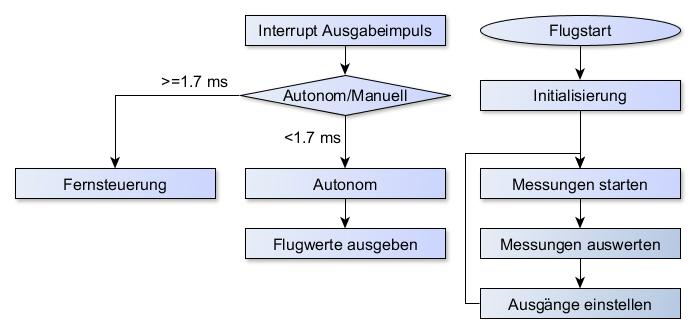
\includegraphics[width = \textwidth]{Bilder/Flussdiagramm}
    \par\end{centering}
    \caption{Flussdiagramm des Gesamtablaufs}
    \label{Flussdiragramm}
  \end{figure}

  Für die weiteren Programmteile wurden jeweils noch detailliertere Flussdiagramme erstellt.

  \subsection{Aufbau des Programms}

  % Erklärung, wer was Aufruft %





%%%%%%%%%%%%%%%%%%%%%%%%%%%%%%%%%%%%%%%%%%%%%%%%%%%%%%%%%%%%%%%%%%%%%%%%%%%%%%%
\section{Navigation}

  \subsection{Technische Planung}



    \subsubsection{Frames}

    % BILD VON LUCAS %


    \subsubsection{Aileron}
    \subsubsection{Elevator}
    \subsubsection{Rudder}

    % Rotationsbild + 2er Komplement %

    \subsubsection{Throttle}

  \subsection{Umsetzung}

    \subsubsection{Vergleichen der Frames}
    Für den Vergleich des aktuellen mit dem letzten Frame, werden zwei \glslink{Struktur}{Strukturen} verwendet, die über folgende Mitglieder verfügt.
    \begin{itemize}
      \item \textbf{num}\\
      ist die ID des getrackten Colorcodes, er besteht aus einer zweistelligen Zahl.
      \item \textbf{pos\_x}\\
      ist die X-Position des Colorcodes. Der Wert bezieht sich auf das Zentrum des Objektes.
      \item \textbf{pos\_y}\\
      ist die Y-Position des Colorcodes. Der Wert bezieht sich auf das Zentrum des Objektes.
      \item \textbf{height}\\
      ist die, vom Ultraschall übergebene Höhe.
      \item \textbf{angle}\\
      ist die Rotation des Colorcodes. Da er zweifarbig ist, kann die PIXY CMUcam5 die Rotation des Objektes feststellen.
    \end{itemize}

    Quelle: \textcolor{red}{TITEL FEHLT \cite{Structs}, das sollte verlegt werden -Lucas}

    Zuerst wird die ID des Colorcodes verglichen, um herauszufinden, ob das Farbobjekt das selbe wie im letzten Frame ist.
    Sollte dies der Fall sein, werden die Koordinaten x und y und die Rotation mit den Werten der älteren Struktur verglichen und gespeichert.
    Diese werden bei den folgenden Funktionen verwendet, um zu überprüfen, ob der Hexacopter die richtige Geschwindigkeit hat.

    \subsubsection{Aileron, Elevator und Rudder anhand der Kameradaten}
    Durch die PIXY CMUcam5 kann die Position des Hexacopters, relativ zu einem Colorcode, festgestellt werden. Gegebenenfalls werden anschließend die Flugparameter verändert.

    \begin{figure} [tbh]
      \begin{centering}
        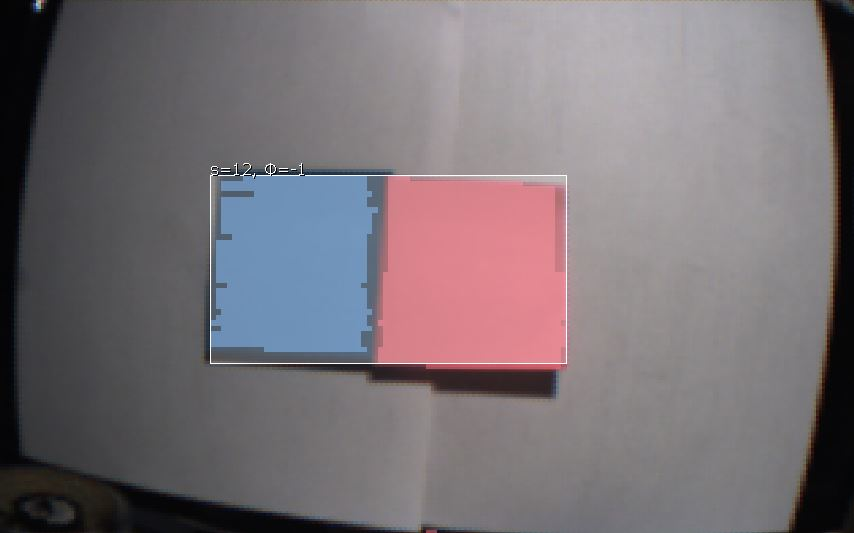
\includegraphics[width = \textwidth]{Bilder/Farbcode_erkannt}
      \par\end{centering}
      \caption{Ein erkannter Farbcode}
      \label{Farbcode_erkannt}
    \end{figure}
    Die Position wird anhand solcher Farbcodes erkannt, im Tischkonzept ist hinterlegt in welcher Reihenfolge der Hexacopter die Farbcodes suchen muss.
    Er fliegt anschließend so lange, bis er über dem aktuellen Farbcode ist, dieser also mittig im Bild ist und sucht darauf den nächsten.


    Die PIXY CMUcam5 XXXXXX % IRGENDWAS MIT X diese länge, y diese länge; %



      \begin{itemize}
        \item \textbf{Überprüfen von Aileron}\\
        Die Überprüfung von Aileron bezieht sich auf die Beschleunigung nach Links und Rechts, was der x-Koordinate entspricht.

        Ziel der Funktion ist es, den Farbcode in die Mitte des Frames zu bekommen. Der Idealzustand befindet sich zwischen 150 und 170.
        Sollte dieser Zustand erreicht werden, bleibt der Wert von Aileron unverändert und der Hexacopter fliegt weiterhin mit einer unveränderten Beschleunigung an der
        x-Koordinate.
        Sollte dies nicht der Fall sein, muss der Wert auf einige Komponenten \textcolor{red}{XXXXX} überprüft werden.
        Wenn der Farbcode zu weit auf der rechten Seite liegt, das bedeutet, wenn der Wert des Mittelpunktes vom Farbobjekt höher als 170 ist,
        muss der Hexacopter nach rechts fliegen, um seine Position zu korrigieren.
        Dabei muss zuerst verglichen werden, ob sich der Hexacopter in die richtige Richtung bewegt. Sollte er in die falsche Richtung
        fliegen, wird der Aileron-Flugparameter gesenkt, dies setzt die Beschleunigung nach Rechts vorraus.
        Wenn die Beschleunigung nach rechts hoch genug ist und die Drohne tatsächlich nach rechts fliegt, wird die Geschwindigkeit überprüft.
        Die Geschwindigkeit wird durch die Differenz der x-Koordinate beider Strukturen herausgefunden. Die Einheit ist in diesem Fall

        \item \textbf{Überprüfen von Elevator}\\
        Position der Farbobjekte (CHECK AILERON \& ELEVATOR)
        Wenn ein Farbobjekt nicht im gewünschten Bereich plaziert ist, muss der Hexacopter weiter nach links oder weiter nach rechts fliegen.
        \item \textbf{Überprüfen von Rudder}\\
        Rotation der Farbojekte (CHECK RUDDER)
        Wenn der Hexacopter über einem Farbobjekt fliegt, soll er kontrollieren, ob der 2-Farbige Code die richtige Rotation hat und sich im richtigen Bereich des Bildschirmes befindet. Wenn diese Informationen richtig sind, darf der Copter zum nächsten Farbobjekt fliegen.
        Durch dieses System könne die genauen Wege vorgegeben werden und können sich durch das gesamte Restaurant verteilen. Durch die Rotation der Codes können auch Kurven eingebaut werden.

        Richtung (CHECK RUDDER)
        Durch die Rotation der Colorcodes, kann der Hexacopter bestimmen, ob er den richtigen Weg und in die richtige Richtung fliegt, wenn er am Weg zurück zur Base ist, muss er den umgekehrten Colorcode verwenden. (Rotation 180Grad)
      \end{itemize}

    \subsubsection{Throttle anhand des Ultraschallsensors}

    Starten und landen auf Landeplattformen (CHECK THROTTLE)
    Der Hexacopter startet und landet auf den mit ebenfalls mit Colorcodes gekennzeichneten Landeplattformen.
    Bei einem Fehler, besteht auch das Landen auf einem beliebigen Fleck

    Höhe korrigieren (CHECK THROTTLE)
    Höhenunterschied zwischen Tisch und Boden

    \subsubsection{Speichern der alten Daten}

    \subsubsection{Ausgabe der Steuersignal}
    Nachdem die Steuersignale berechnet und korrigiert wurden müssen diese an den Hexacopter ausgegeben werden. Dies muss periodisch alle $\SI{20}{\milli\second}$ geschehen.
    Der Flightcontroller erkennt jeweils die einzelnen Impulse und steuert die Rotoren entsprechend an.

    Diese Impulse werden Interrupt-gesteuert ausgegeben, der Interrupt wird von dem Gear-Pin erzeugt welcher gleichzeitig für den Flugmodus verantwortlich ist.

    \lstset{language = c}
    \begin{lstlisting}
interrupt void Isr() {
  if(CCP1IF == 1) {
    CCP1IF = 0;
    T1CONbits.TMR1ON = 0;
    SignalOut();
    NOP();
  }
  if(TMR3GIF == 1) {
    TMR3GIF = 0;
    ModeCheck();
    SignalOut();    /* initial call after remaining break to 20 ms
                     * starts with Aileron (needs to be set in last
                     * case statement, case 0) following delays will
                     * be processed by the previous routine */
    pulsecounter++;
  }
}

void SignalOut(void) {
  switch(pin_out) {
    case 'A': {
      A = 1;
      Delay(a_actors[0].aile);
      pin_out = 'E';
      break;
    }case 'E': {
      A = 0;
      E = 1;
      Delay(a_actors[0].elev);
      pin_out = 'T';
      break;
    }
    \end{lstlisting}
    Die weiteren Signale (Throttle und Rudder) werden auf die gleiche Weise ausgegeben.
    Die Delay-Funktion stellt die Compare-Einehit so ein, dass nach der gewünschten Pulsdauer des Ausgangs ein Interrupt hervorgerufen wird.

%%%%%%%%%%%%%%%%%%%%%%%%%%%%%%%%%%%%%%%%%%%%%%%%%%%%%%%%%%%%%%%%%%%%%%%%%%%%%%%
\section{Objekterkennung}

  \subsection{Technische Planung}

  \subsection{Umsetzung}

  \subsection{Herausforderungen und Lösungen}

%%%%%%%%%%%%%%%%%%%%%%%%%%%%%%%%%%%%%%%%%%%%%%%%%%%%%%%%%%%%%%%%%%%%%%%%%%%%%%%
\section{Sicherheit}

  \subsection{Technische Planung}

  \subsection{Umsetzung}

  \subsection{Herausforderungen und Lösungen}

%%%%%%%%%%%%%%%%%%%%%%%%%%%%%%%%%%%%%%%%%%%%%%%%%%%%%%%%%%%%%%%%%%%%%%%%%%%%%%%
\section{Systemausfall}

  \subsection{Technische Planung}

  \subsection{Umsetzung}

  \subsection{Herausforderungen und Lösungen}
